The purpose of the functions related to the query language is to work with huge BioPAX files and extract from the BioPAX documents only the information that is of interest. For this part, we will use the apoptosis example initially extracted from Reactome database: Apoptosis.owl. This set of functions can be used with big pathway databases already exported to BioPAX: Reactome, BioCyc, NetPath (see http://www.biopax.org for the complete list).

\subsection{Generate Index}
\textbf{Plugins$\Rightarrow$BiNoM BioPAX 3 Query$\Rightarrow$Generate Index}\\
Using this function BiNoM maps the content of BioPAX file onto a labeled graph (referred to as index). It creates an *.xgmml file from an *.owl one (figure~\ref{Generate_BioPAX_Index}). For the definition of BioPAX index, see section~\ref{Standard_BioPAX_Interfaces}.
\begin{figure}[h]
\centering
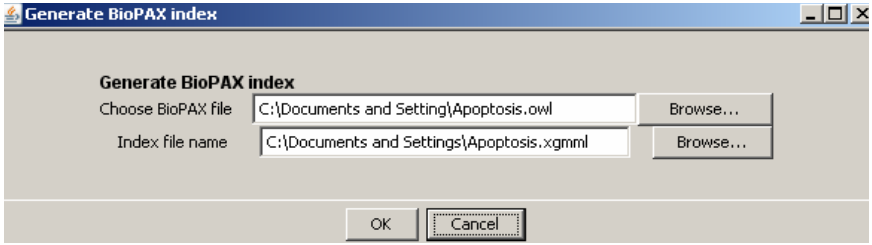
\includegraphics[width=18 cm]{graphics/Generate_BioPAX_Index}
\caption{Generate BioPAX Index.}
\label{Generate_BioPAX_Index}
\end{figure}

\subsection{Load Index}
\textbf{Plugins$\Rightarrow$BiNoM BioPAX 3 Query$\Rightarrow$Load Index}\\
Once the xgmml is created, it can be loaded into memory. The index is global object, i.e. only one index can be used at a time.Load Index loads the index file from xgmml format (figure~\ref{Load_Index_Dialog}).\\\\
\begin{figure}[h]
\centering
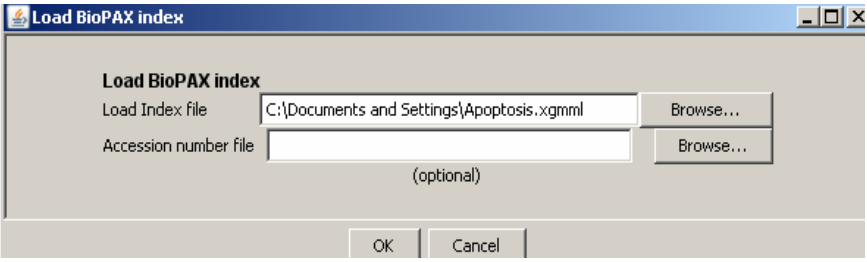
\includegraphics[width=18 cm]{graphics/Load_Index_Dialog}
\caption{Load Index dialog.}
\label{Load_Index_Dialog}
\end{figure}
Together with the index, you can also upload a tab-delimited “accession number file” which corresponds to a list of synonyms for the genes/proteins ids used in a network (see an example of the content of some accession number file at figure~\ref{Accession_Number_File}). An entity in the index can be identified by its id, by any XREF attribute (see section~\ref{Standard_BioPAX_Interfaces}), by node name, or by any synonym from the accession table (if it is provided).
\begin{figure}[h]
\centering
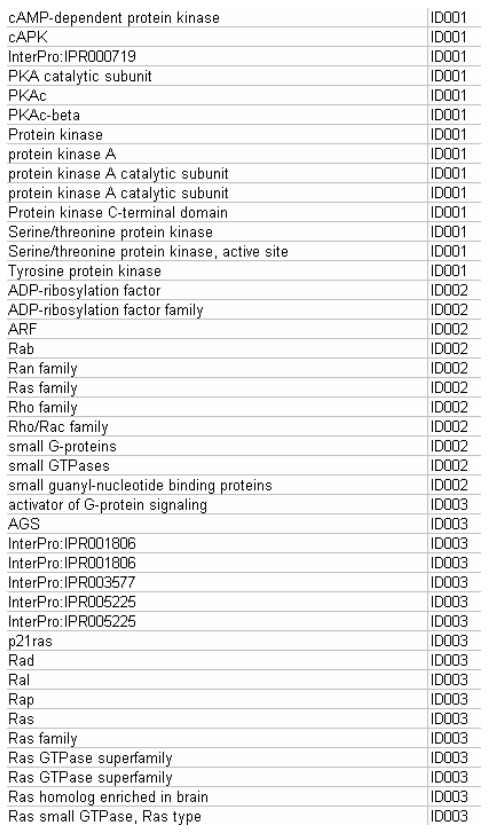
\includegraphics[width=8 cm]{graphics/Accession_Number_File}
\caption{Example of accession Number file. First column is a synonym (which can have structure $\textless database\textgreater :\textless standard_id\textgreater)$, the second column is the id used inside the BioPAX file.}
\label{Accession_Number_File}
\end{figure}

\subsection{Display Index Info}
\textbf{Plugins$\Rightarrow$BiNoM BioPAX 3 Query$\Rightarrow$Display Index Info}\\
This command opens a window indicating the name of the graph, the name of the file, the accession number file, when available, the number of records, and the various statistics of the index: number of publications, proteins, physicalEntities, complexes, biochemical reactions, pathways, pathwaySteps, catalyses, and modulations (necessary proteins for catalyses). See figure~\ref{BioPAX_Index_Info}.
\begin{figure}[h]
\centering
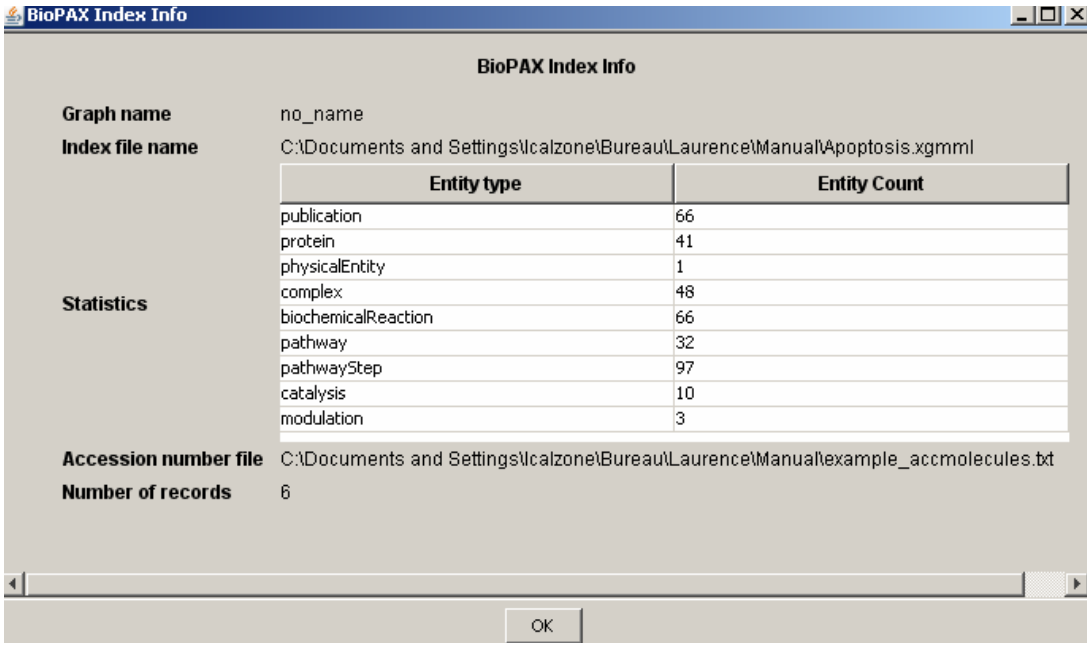
\includegraphics[width=18 cm]{graphics/BioPAX_Index_Info}
\caption{Display Index info.}
\label{BioPAX_Index_Info}
\end{figure}

\subsection{Select Entities}
\textbf{Plugins$\Rightarrow$BiNoM BioPAX 3 Query$\Rightarrow$Select Entities}\\
The BioPAX document is often too big to find the protein or gene that needs to be studied. To access it easily and rapidly, it is possible to find the component directly with this command and build a specific network around that molecule.\\\\
For example, in Apoptosis.xgmml, we choose to find the caspases 8 and extend the network around it. When choosing Plugins => BiNoM BioPAX Query => Select entities from the index, a dialog window pops up and offers the possibility to find a protein or a gene by its name or id or XREF attribute or synonym, from the current network when a network is already opened, or from the list of identities associated with the BioPAX index (figure~\ref{Select_entities_from_index}).\\\\
For our example, we choose the second option. To increase the probability to find the protein in the list, we propose, in figure~\ref{Select_entities_from_index}, three different versions of the same name: CASP8, Caspase8 or caspases\_8, all separated by space (the separator can be also comma and semi-colon or line-break symbol). One of them (CASP8) corresponds to the name from the BioPAX list and a new network is created with only one protein, CASP8 (= MCH5 in the index), at the center of it. The other ones were not found (see output in figure~\ref{xxx}). It is also possible to select more than one entity, in this case, the components all appear in the same window.\\\\
The output is chosen to appear in a new network (selection is made at the bottom of the dialog window in figure~\ref{Select_entities_from_index}) but it is also an option to view several genes or proteins in the same network by checking “output in the current network”.\\\\
\begin{figure}[h]
\centering
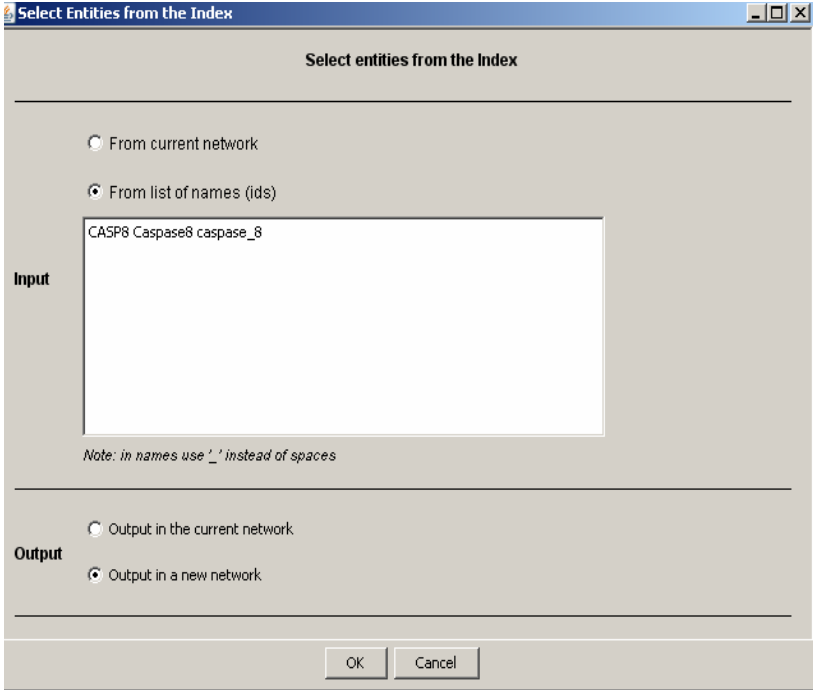
\includegraphics[width=14 cm]{graphics/Select_entities_from_index}
\caption{Select entities from the index.}
\label{Select_entities_from_index}
\end{figure}
A network is created with only one node, caspase 8, called MCH5 in the index. Note that for this part, it is advised to use the BiNoM BioPAX visual style to view the resulting network.

\subsection{Standard Query}
\textbf{Plugins$\Rightarrow$BiNoM BioPAX 3 Query$\Rightarrow$Standard Query}\\
This command proceeds through a series of actions that will extend or make the studied network more specific to the user’s needs.\\\\
Let’s start with diverse queries from the network created for the Caspase 8 entity. A dialog window opens as figure~\ref{Standard_Query_Dialog}.\\\\
\begin{figure}[h]
\centering
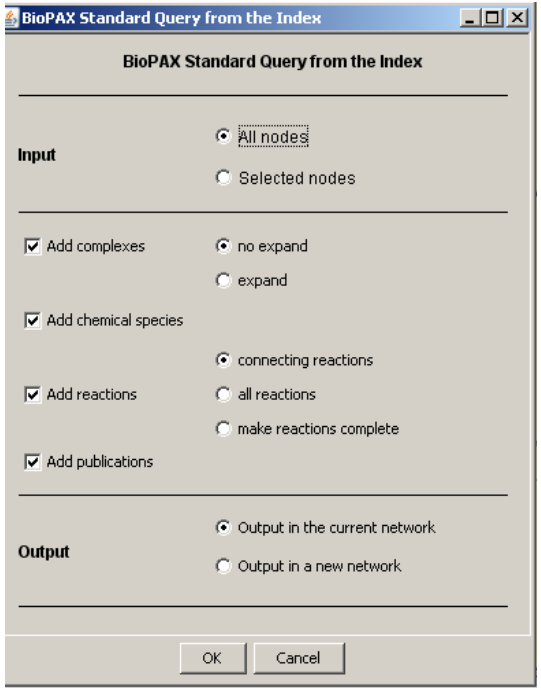
\includegraphics[width=12 cm]{graphics/Standard_Query_Dialog}
\caption{BioPAX Standard Query: dialog window.}
\label{Standard_Query_Dialog}
\end{figure}
All the options proposed in the dialog window (figure~\ref{Standard_Query_Dialog}) are listed here:
\subsubsection{In the input section}
All nodes / Selected nodes: In the network, you can submit queries that concern all the nodes in the network or only the selected nodes (highlighted in yellow). 
\subsubsection{Once you decide on which proteins you wish to work, you can:}
\begin{itemize}
\item Add complexes
\begin{itemize}
\item “no expand” adds only the homodimers of the molecule (figure~\ref{Standard_Query_Add_complexes}a). If several proteins were queried, then all hetero-dimers in which all the proteins participate would appear.
\item “expand” adds all the complexes in which MCH5 is involved (figure~\ref{Standard_Query_Add_complexes}b). The green arrow with a diamond ending represents the inclusion of one protein in a complex form.
\end{itemize}
\begin{figure}[h]
\centering
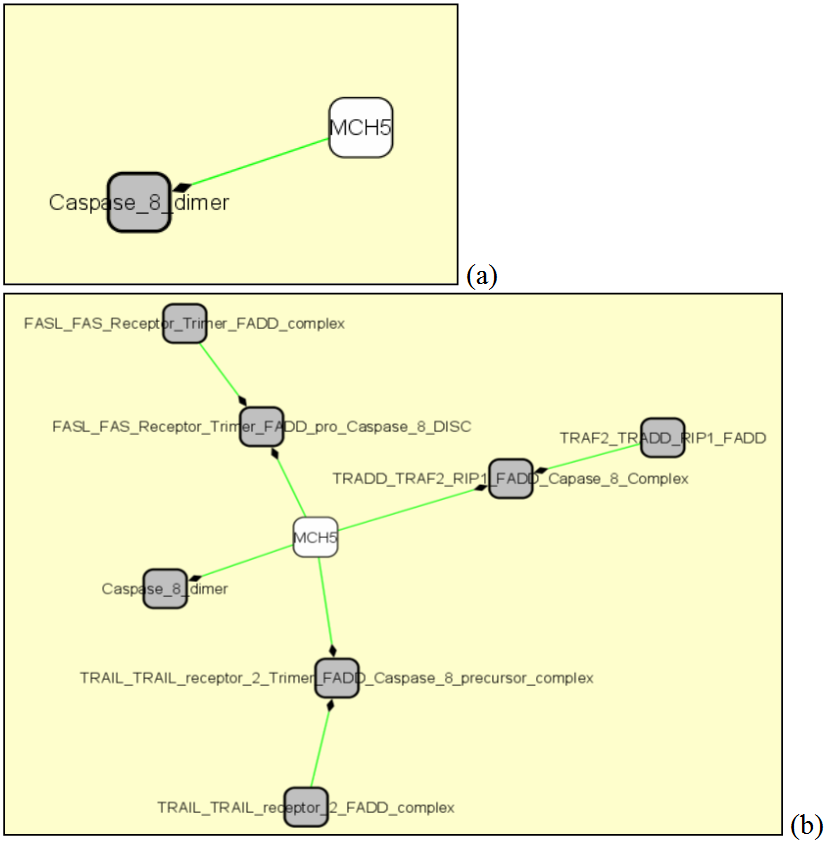
\includegraphics[width=18 cm]{graphics/Standard_Query_Add_complexes}
\caption{BioPAX Standard Query: Add complexes with (a) the « no expand” or (b) “expand” option.}
\label{Standard_Query_Add_complexes}
\end{figure}
\item Add chemical species\\
This function adds, for each species, the cellular location and its specified modifications. It is linked to the protein with a grey edge (see figure~\ref{Standard_Query_Chemical_species}).
\begin{figure}[h]
\centering
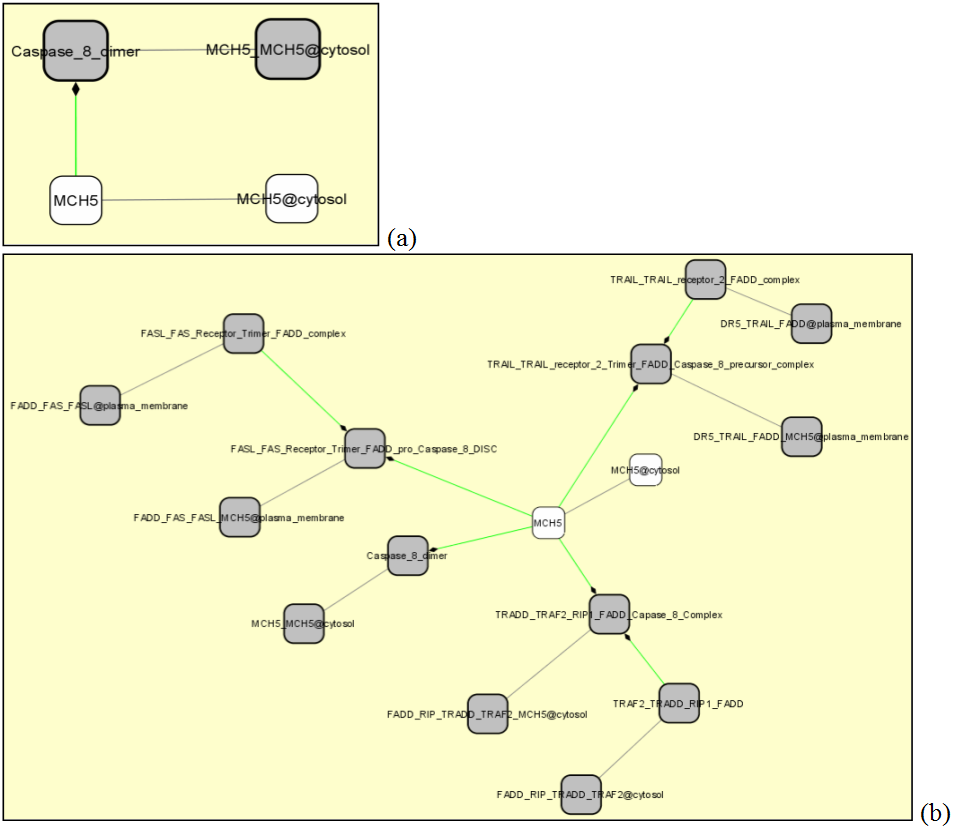
\includegraphics[width=18 cm]{graphics/Standard_Query_Chemical_species}
\caption{Chemical species. Cellular locations of all forms of MCH5.}
\label{Standard_Query_Chemical_species}
\end{figure}
\item Add reactions
\begin{itemize}
\item “connecting reactions” connects all present species that have common reactions (connected by a yellow node in figure~\ref{Standard_Query_All_connecting_reactions}).
\begin{figure}[h]
\centering
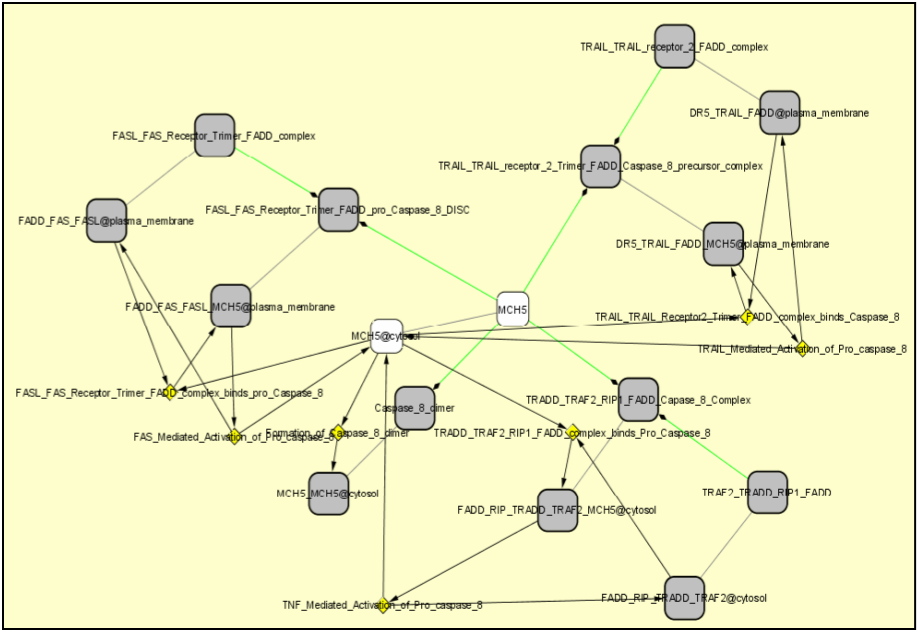
\includegraphics[width=18 cm]{graphics/Standard_Query_All_connecting_reactions}
\caption{Adding reactions: example when all connecting reactions.}
\label{Standard_Query_All_connecting_reactions}
\end{figure}
\item “all reactions” includes all the reactions involving the chemical species (figure~\ref{Standard_Query_Adding_all_reactions}).
\begin{figure}[h]
\centering
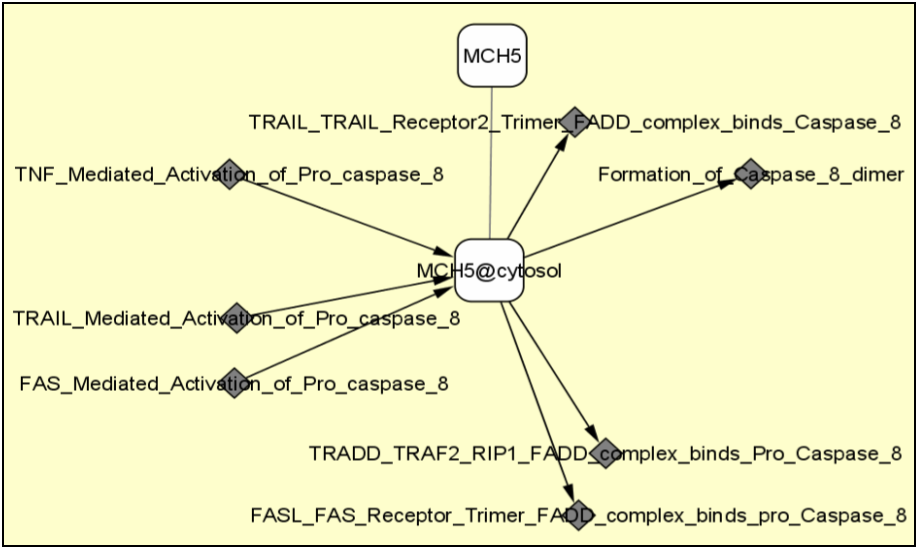
\includegraphics[width=18 cm]{graphics/Standard_Query_Adding_all_reactions}
\caption{Adding reactions: example adding all reactions.}
\label{Standard_Query_Adding_all_reactions}
\end{figure}
\item “make reactions complete” adds all the sources and targets of the reactions (figure~\ref{Standard_Query_Making_reactions_complete}) listed in the BioPAX index, including, for example, the pathway nodes and publications links.
\begin{figure}[h]
\centering
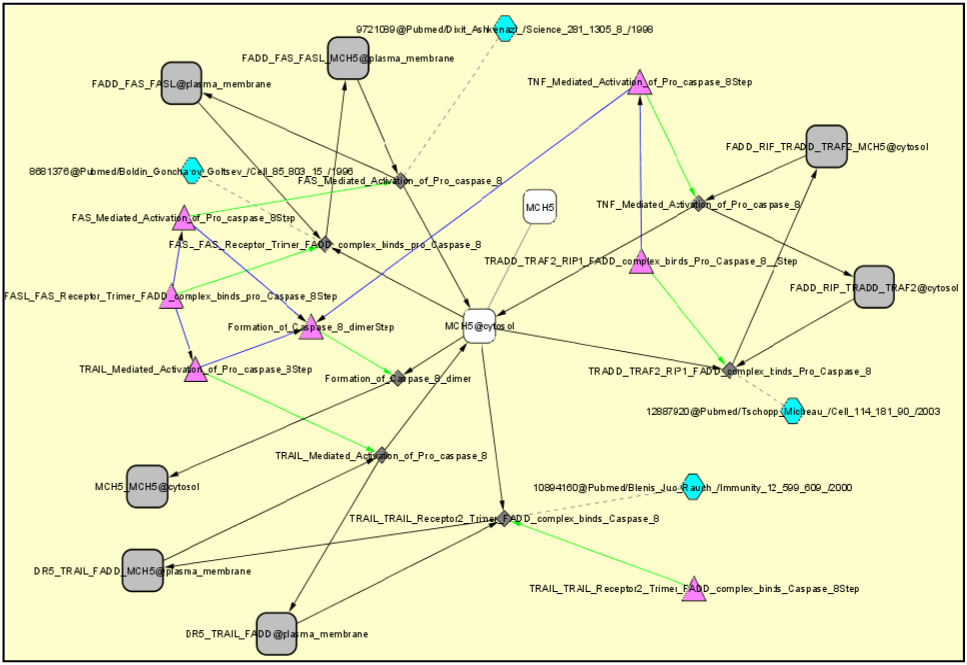
\includegraphics[width=18 cm]{graphics/Standard_Query_Making_reactions_complete}
\caption{Adding reactions: example when making the reactions complete.}
\label{Standard_Query_Making_reactions_complete}
\end{figure}
\end{itemize}
\item Add publications\\
When available, this function adds all the references associated with a reaction (see figure~\ref{Standard_Query_Adding_publications}).
\begin{figure}[h]
\centering
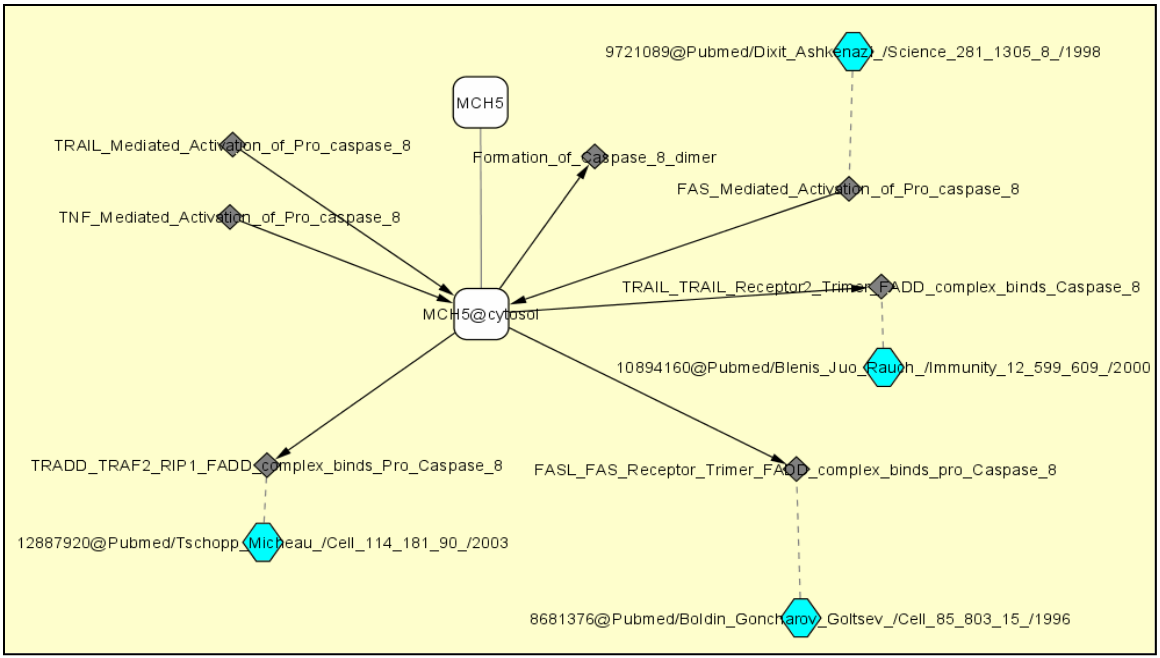
\includegraphics[width=18 cm]{graphics/Standard_Query_Adding_publications}
\caption{Adding publications.}
\label{Standard_Query_Adding_publications}
\end{figure}
\end{itemize}
\subsubsection{Output}
The result of the queries can be seen either in the current network or in a new network.

\parbox{\textwidth}{
\subsection{Index Path Analysis}
\textbf{Plugins$\Rightarrow$BiNoM BioPAX 3 Query$\Rightarrow$Index Path Analysis}\\
This command finds the directed or non-directed, shortest, optimal or suboptimal, non intersecting paths with a pre-defined number of intermediaries in an index file. Note that the species need to be selected on a graph before this query.\\\\
This part of the query engine uses the same algorithms and options as Path analysis dialog (see section~\ref{Path_Analysis}), however, with the network (index) kept completely in memory, without explicit visualization. Moreover, the network is slightly modified before this type of query: in particular, all non-directed edges (of CONTAINS, SPECIESOF and some other types) are represented as bi-directional, some nodes (publications and, optionally, smallMolecules) are removed.\\\\
For example, the following steps
\begin{enumerate}
\item Select Entities: specify CASP8 and FAS proteins.
\item Select the two nodes.
\item Index Path analysis: Find all non-intersecting paths.
\item BiNoM Analysis: Extract Reaction Network.
\end{enumerate}
produce the following network connecting CASP8 and FAS proteins (it also involves FADD because it complexes with FAS and CASP8 on the membrane). See figure~\ref{Index_Path_Analysis}.
}
\begin{figure}[h]
\centering
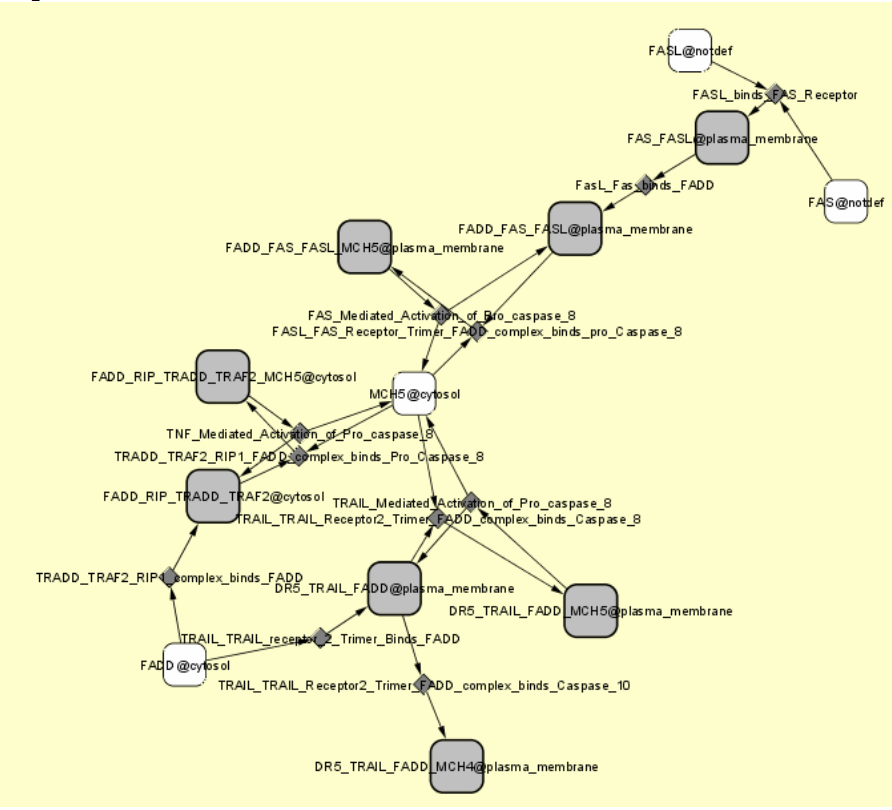
\includegraphics[width=18 cm]{graphics/Index_Path_Analysis}
\caption{Index path Analysis with CASP8 and FAS.}
\label{Index_Path_Analysis}
\end{figure}

\subsection{View Query Log}
\textbf{Plugins$\Rightarrow$BiNoM BioPAX 3 Query$\Rightarrow$}\\
In this window (figure~\ref{BioPAXViewQueryLogDialog}), are recapitulated all the queries done during the session.
\begin{figure}[h]
\centering
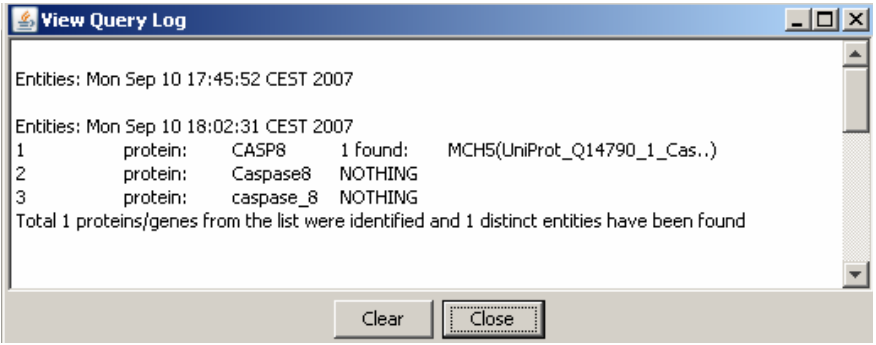
\includegraphics[width=18 cm]{graphics/BioPAXViewQueryLogDialog}
\caption{View Query Log Dialog}
\label{BioPAXViewQueryLogDialog}
\end{figure}